% A typical element of the algebra generated by axis-aligned boxes in
% the plane: a finite union of rectangles (here an L-shaped union and
% a separate box).
% Source: book/tex/measure/caratheodory.tex (§ Algebras) — asy figure.
\documentclass[border=2mm]{standalone}
\usepackage{tikz}
\begin{document}
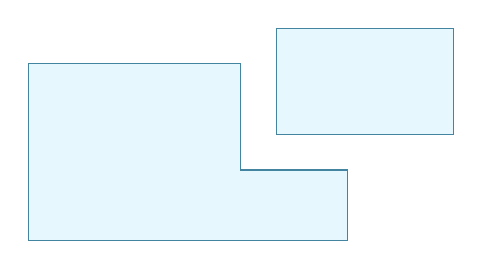
\begin{tikzpicture}[scale=0.45]
  \filldraw[fill=cyan!10, draw=cyan!60!black]
    (0,0) -- (9,0) -- (9,2) -- (6,2) -- (6,5) -- (0,5) -- cycle;
  \filldraw[fill=cyan!10, draw=cyan!60!black]
    (7,3) rectangle (12,6);
\end{tikzpicture}
\end{document}
